\subsection{Reciprocal Kit Build}
\begin{frame}[allowframebreaks]{Reciprocal Kit Build (RKB)}
    
    %\href{run:/path/nameofvideo.mp4}{Click for video}
     \begin{figure}[tb]
         \begin{center}
         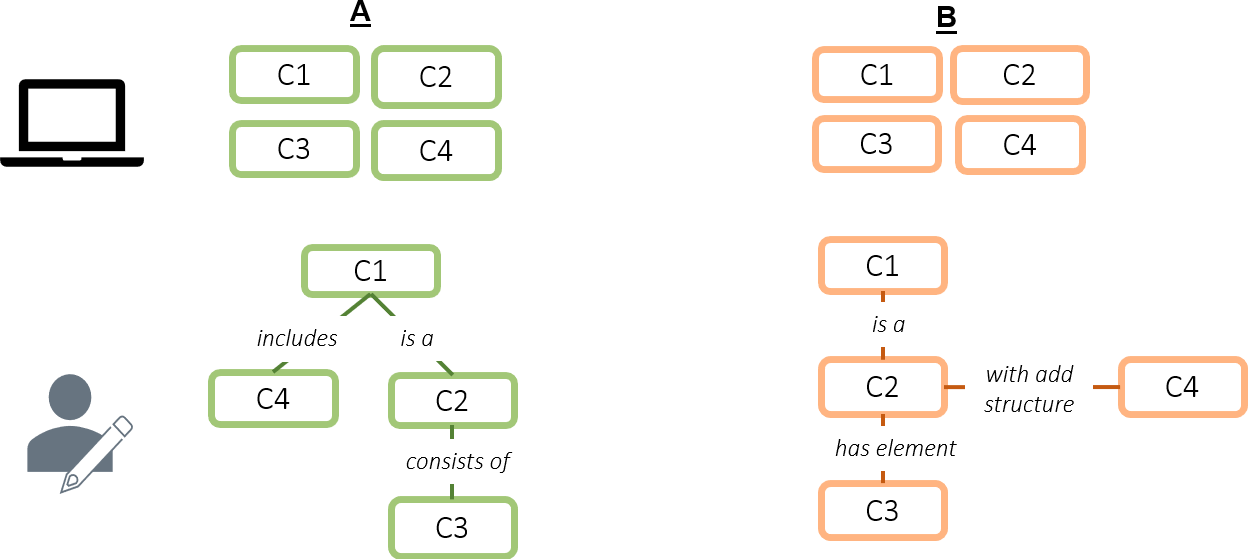
\includegraphics[width=100mm]{images/RKB_p1.pdf}
         \end{center}
         \caption{\emph{Individual phase} -- Initial map construction}
         \label{intro::rkb_p1}
     \end{figure}
    
     \begin{figure}[tb]
         \begin{center}
             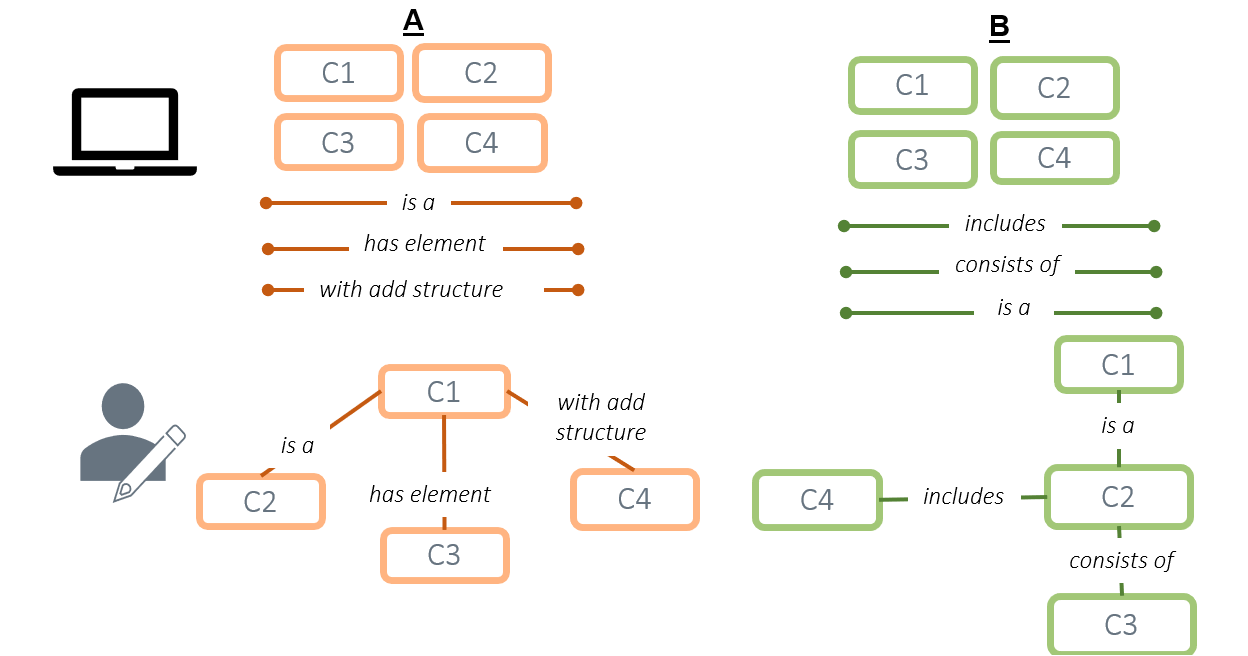
\includegraphics[width=100mm]{images/RKB_p2.pdf}
         \end{center}
         \caption{\emph{Individual phase} -- Re-constructional map building}
         \label{intro::rkb_p2}
     \end{figure}
    
     \begin{figure}[tb]
         \begin{center}
             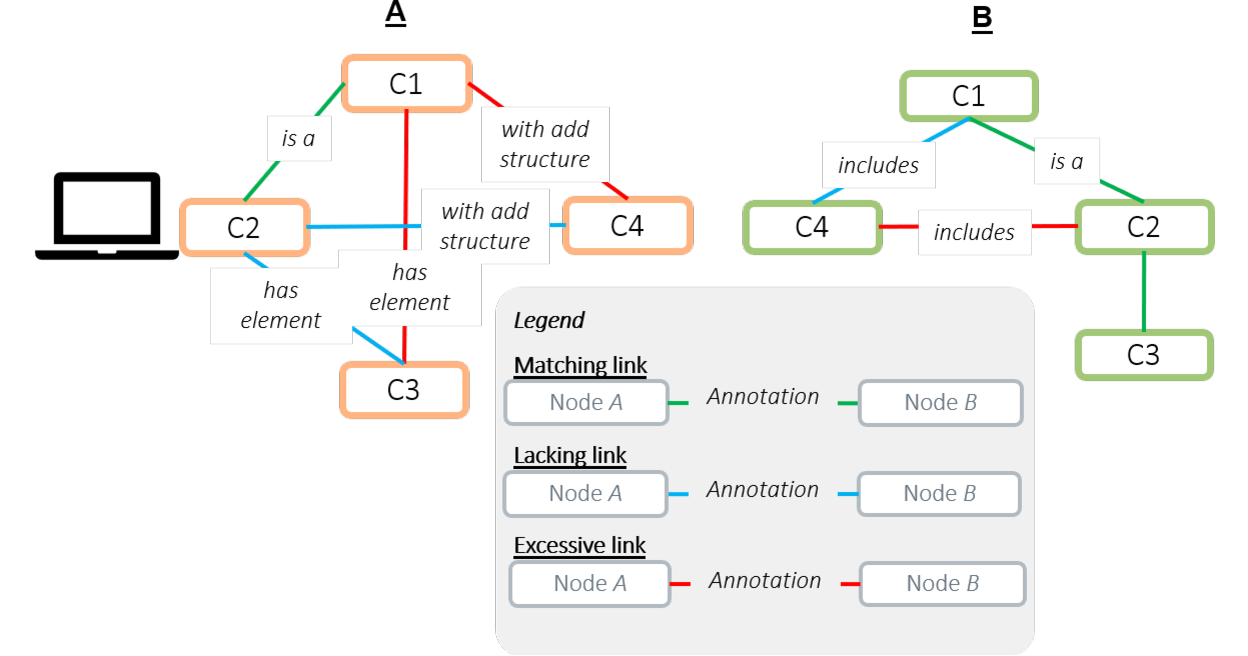
\includegraphics[width=100mm]{images/RKB_p3.pdf}
         \end{center}
         \caption{\emph{Collaborative phase} -- Visualization of map similarities and differences \& group discussion}
         \label{intro::rkb_p3}
     \end{figure}
    
     \begin{figure}[tb]
         \begin{center}
             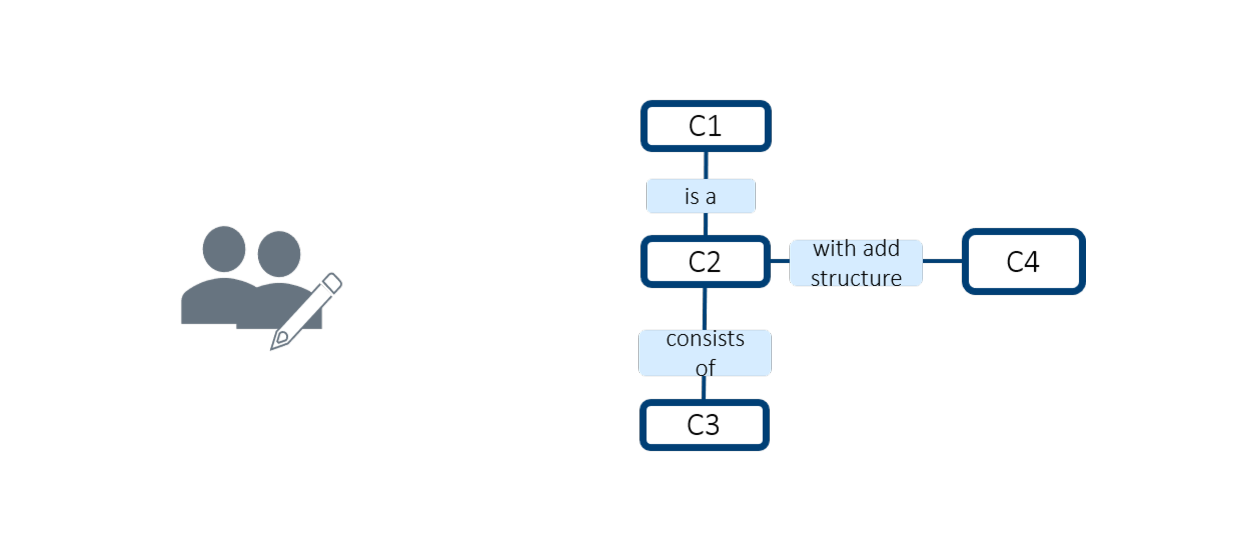
\includegraphics[width=100mm]{images/RKB_p4.pdf}
         \end{center}
         \caption{\emph{Collaborative phase} -- Group map construction}
         \label{intro::rkb_p4}
     \end{figure}
\end{frame}

\subsection{Experimental procedures}

\begin{frame}{Experimental settings}
\begin{itemize}
    \item Course name: Linear Algebra class of 2018
    \item Selected topics: General Vector Space and Inner Product Space
    \item Fourteen concepts selected as predefined nodes
    \item Group formation: dyad (pair), selected freely by the students
    \item Location: computer laboratory, participants sit next to their partner
\end{itemize}

\begin{figure}[tb]
    \begin{center}
            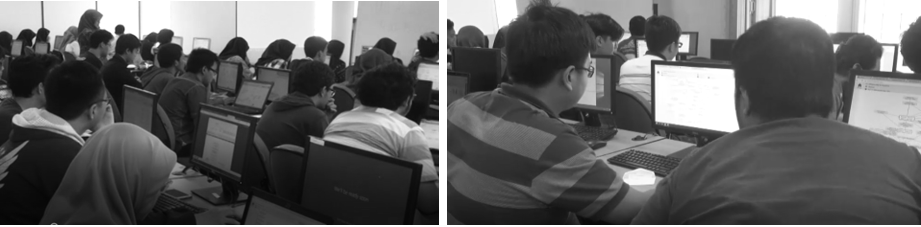
\includegraphics[width=100mm]{images/classroom_situation.pdf}
        \end{center}
        \caption{Classroom situation}
        \label{intro::classroom}
    \end{figure}

\end{frame}

\begin{frame}{The learning activities during experiment: the individual phase}
    \begin{figure}[tb]
        \begin{center}
            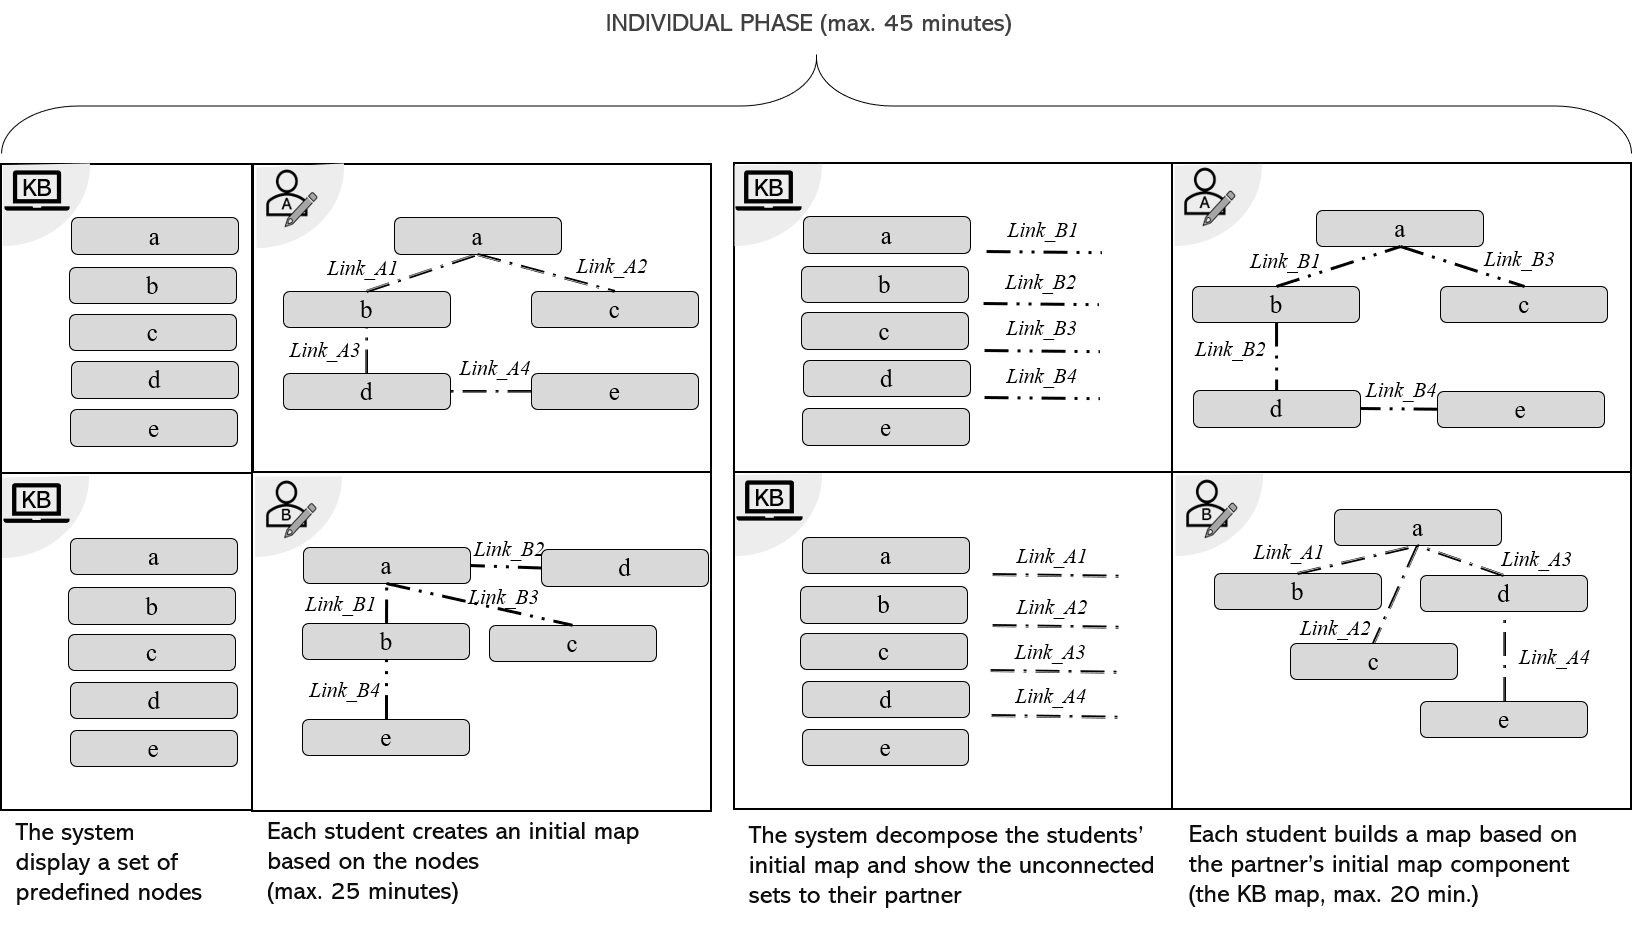
\includegraphics[width=90mm]{images/method_ind_phase_RKB.pdf}
        \end{center}
        \caption{Timeline of students' activities (individual phase)}
        \label{method::rkb_ind_phase}
    \end{figure}
    
\end{frame}
\begin{frame}{The learning activities during experiment: the collaborative phase}
    \begin{figure}[tb]
        \begin{center}
            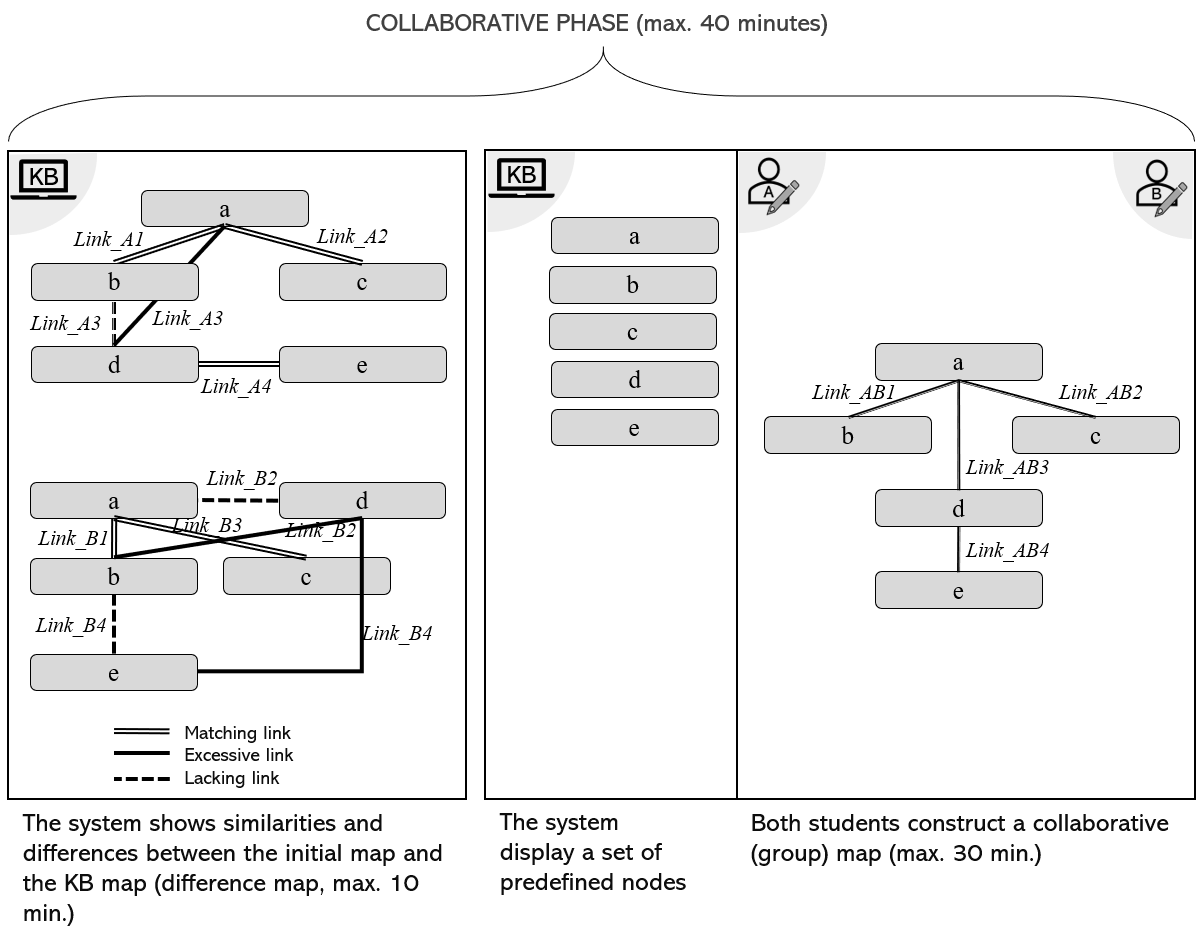
\includegraphics[width=75mm]{images/method_collab_phase_RKB.pdf}
        \end{center}
        \caption{Timeline of students' activities (collaborative phase)}
        \label{intro::rkb_collab_phase}
    \end{figure}
    {\tiny **Note: Three days after the experiment, the teacher gave feedback to the students. \\
    The consent form to participate and a survey regarding students' affective response
    toward the activities were also collected afterward. }

\end{frame}
    
    % \begin{table}[tb]
    % \begin{center}
    % \begin{tabular}{p{2.5cm}|p{5.5cm}|p{2cm}}%{c|c|c} %#{ | m{5em} | m{1cm}| m{1cm} | }
    % \hline
    % Phase & Students' Activity & Duration\\
    % \hline
    % Introduction & Kit-Build practice & 5 min.\\
    % Individual & (a) Create a concept map based on the predefined concepts (first map) & 25 min.\\
    % & (b) Create a re-constructional map based on the partner's first map components (second map) & 20 min.\\
    % Collaborative & (a) Discussion on shared and difference maps & 10 min.\\
    % & (b) Create a group concept map  (third map) & 30 min.\\
    % \hline
    % \end{tabular}
    % \end{center}
    % \caption{\label{tab:exp_setting} Timeline of students' activities during experiment}
    % \end{table}
 


\subsection{Participants characteristics}

% \begin{frame}{Methods}

% \begin{itemize}
%   \item Participants and context of study
%   \item Experimental procedures
%   \item Data collection
% \end{itemize}

% \end{frame}

\begin{frame}{Participants}

\begin{itemize}
    \item <1-> \textcolor{blue}{Forty-four students} of Linear Algebra class
    \item <1-> Majored in \textcolor{blue}{Computer Science or Information System} at a public university in Indonesia
    \item <1> \textcolor{blue}{73\%} of them are \textcolor{blue}{male} students ($n = 32$)
    \item <1> Most of them were the first year students in their second term (ages of 18-22 years old)
    \item <2-> They had \textcolor{blue}{experiences in various collaborative learning} activities
    \item <2-> They were \textcolor{blue}{familiar with concept mapping} and used to create a concept map from scratch
\end{itemize}

\end{frame}
